\documentclass[11pt,a4paper]{article}

% Packages
\usepackage[utf8]{inputenc}
\usepackage[spanish, es-tabla]{babel}
\usepackage{caption}
\usepackage{listings}
\usepackage{adjustbox}
\usepackage{enumitem}
\usepackage{boldline}
\usepackage{amssymb, amsmath,amsthm}
\usepackage[margin=1in]{geometry}
\usepackage{xcolor}
\usepackage{soul}
\usepackage{upgreek}
\usepackage{float}

% Meta
\title{Entrega 3}
\author{José Antonio Álvarez}
\date{\today}

% Custom
\providecommand{\abs}[1]{\lvert#1\rvert}
\setlength\parindent{0pt}
% Redefinir letra griega épsilon.
\let\epsilon\upvarepsilon
% Fracciones grandes
\newcommand\ddfrac[2]{\frac{\displaystyle #1}{\displaystyle #2}}
% Primera derivada parcial: \pder[f]{x}
\newcommand{\pder}[2][]{\frac{\partial#1}{\partial#2}}

\begin{document}

\maketitle

\textbf{Ejercicio 27.} Construir expresiones regulares para los siguientes lenguajes sobre el alfabeto $\{0,1\}$: 

\begin {enumerate} 

\item Palabras en las que el número de símbolos 0 es múltiplo de 3.
	
$$(1^*01^*01^*01^*)^*$$
	
\item Palabras que contienen como subcadena a 1100 ó a 00110.
	
$$(1+0)^*(1100 + 00110)(1+0)^*$$
	
\item Palabras en las que cada cero forma parte de una subcadena de 2 ceros y cada 1 forma parte de una subcadena de 3 unos. \\

Por este enunciado entiendo que se refiere a que para cada 0 existe una subcadena de longitud 2 contenida en la palabra a la que pertenece el 0. Es decir, la subcadenas serán de 2 ceros o más, ya que para cada 0 dentro de dicha cadena podemos encontrar una subcadena de dos ceros. De igual forma apra los unos: 

$$(00^+ + 111^+)^*$$

\item Palabras en las que el número de ocurrencias de la subcadena 011 es menor o igual que el de ocurrencias de la subcadena 110. \\

Este lenguaje no es regular y por tanto no se puede construir una expresión regular para él. Veamos que no lo es por el lema de bombeo.

Sea $L$ el lenguaje definido en el enunciado y $u = (011)^n(110)^n \in L$. Tomando $v = (011)^N$ y $w = (110)^N$, tomando $i=2\  \forall n \in N$, $$ v^iw = (011)^{2n}(110)^n \notin L$$.

Como esto es válido para todo $n$, $L$ no es regular. 

\end{enumerate}

\textbf{Ejercicio 29.} Encuentra para cada uno de los siguientes lenguajes una gramática de tipo 3 que lo genere o un autómata finito que lo reconozca: 

\begin{enumerate}
\item $L_1 = \{ u \in \{0,1\}^* : u \text{ no contiene la subcadena } 0101 \}$
\item $L_2 = \{ 0^i1^j0^k : i \geq 1, j \geq 2, k \geq 0, i \text{ impar}, k \text{ múltiplo de } 3  \}$
\end{enumerate}
Diseña el AFD minimal que reconoce el lenguaje $(L_1 \cap L_2)$. \\

Primero veamos que $L_2 \subset L_1$ y que por tanto $L_2 = (L_1 \cap L_2)$. Sin embargo esto es obvio: una palabra de la forma $0^i1^j0^k$ no puede contener a la sucadena 0101. Por tanto nos limitaremos a dar un AFD minimal para cada lenguaje.

\begin{figure}[H]
	\centering
	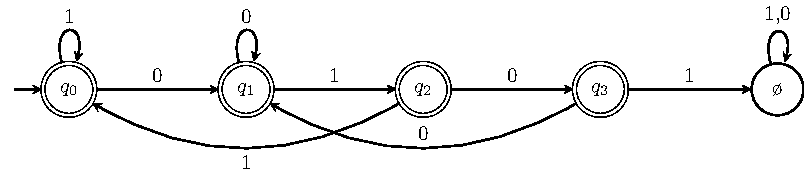
\includegraphics[width=0.8\textwidth]{afd_29_1}
	\caption{Autómata finito determinista minimal que reconoce $L_1$.}
\end{figure}

\begin{figure}[H]
	\centering
	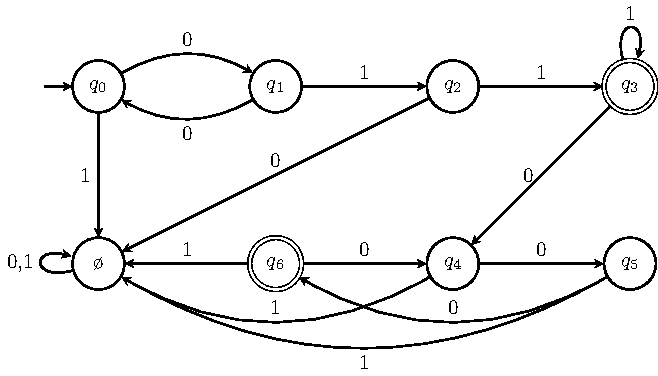
\includegraphics[width=0.8\textwidth]{afd_29_2}
	\caption{Autómata finito determinista minimal que reconoce $L_2$.}
\end{figure}

\textbf{Ejercicio 45.} Sea el alfabeto $A = \{0, 1, +, =\}$, demostrar que el lenguaje
$$ADD = \{x = y + z \ |\  x, y, z \text{ son números en binario, y } x  \text { es la suma de } y \text{ y } z\}$$
no es regular. \\

Lo mostraremos por el lema de bombeo. Sea $z = [1^N + 0 = 1^N] \in ADD$. Tomando $v = 1^N$ y $w = [+\ 0 = 1^N]$, $i=2\ \forall n \in N$:
$$v^iw = [1^{2N} + 0 = 1^N] \notin ADD$$.

Como esto es válido para todo $n$, $ADD$ no es regular. \\

\textbf{Ejercicio 46.} Si $L_1$ y $L_2$ son lenguajes sobre el alfabeto $A$, entonces la \emph{mezcla perfecta} de estos lenguajes se define como el lenguaje:
$$L_3 = \{w \ |\ w = a_1b_1...a_kb_k \text{ donde } a_1...a_k \in L_1, b_1...b_k \in L_2, a_i,b_i \in A\}$$

Demostrar que si $L_1$ y $L_2$ son regulares, entonces la mezcla perfecta de $L_1$ y $L_2$ es regular. \\

Para resolver este ejercicio utilizaremos el teorema de Myhill-Nerode. Sean $\equiv_1$ y $\equiv_2$ las relaciones de equivalencia definidas por el teorema en $L_1$ y $L_2$ respectivamente. Como $L_1$ y $L_2$ son regulares tienen un número de clases de equivalencia finito: $n_1$ y $n_2$ respectivamente. \\

Por la forma en la que está definida la \emph{mezcla perfecta} podemos suponer que unicamente uniremos palabras de $L_1$ y $L_2$ que tengan la misma longitud y unicamente obtendremos palabras pares. Es decir, $L_3 \subset P(A^*) = \{u \in A^* : |u| \text{ es par}\} \ \forall L_1,L_2 \subset A^*$. \\

Numeremos ahora las clases de equivalencia de $L_1$: $[A_i], i \in \{1,...,n_1\}$, y de la misma forma para $L_2$: $[B_i], i \in \{1,...,n_2\}$. \\

Definimos a continuación una nueva relación de equivalencia en $L_3$, $\equiv_3$ de forma tal que:

$$ a = a_1...a_k \equiv_3 b = b_1...b_k \leftrightarrow \begin{cases} a_1...a_{k-1} \equiv_1 b_1...b_{k-1} \\ a_2...a_k \equiv_2 b_2...b_k \end{cases} $$

Donde $k$ es par porque $a,b \in L_3 \subset P(A^*)$. Podemos ver de forma clara que es una relación de equivalencia:

\begin{itemize}
\item Reflexividad:

$$ a \equiv_3 a \leftrightarrow \begin{cases} a_1...a_{k-1} \equiv_1 a_1...a_{k-1} \\ a_2...a_k \equiv_2 a_2...a_k \end{cases} $$

Lo cual se verifica por la reflexividad de $\equiv_1$ y $\equiv_2$.

\item Simetría:

$$ a \equiv_3 b \leftrightarrow \begin{cases} a_1...a_{k-1} \equiv_1 b_1...b_{k-1} \\ a_2...a_k \equiv_2 b_2...b_k \end{cases}  \leftrightarrow \begin{cases} b_1...b_{k-1} \equiv_1 a_1...a_{k-1} \\ b_2...b_k \equiv_2 a_2...a_k \end{cases} \leftrightarrow b \equiv_3 a$$

\item Transitividad:

$$ \begin{cases} a \equiv_3 b \\ b \equiv_3 c \end{cases} \leftrightarrow \begin{cases} a_1...a_{k-1} \equiv_1 b_1...b_{k-1} \\ a_2...a_k \equiv_2 b_2...b_k \\ b_1...b_{k-1} \equiv_1 c_1...c_{k-1} \\ b_2...b_k \equiv_2 c_2...c_k \end{cases}  \implies \begin{cases} a_1...a_{k-1} \equiv_1 c_1...c_{k-1} \\ a_2...a_k \equiv_2 c_2...c_k \end{cases} \leftrightarrow a \equiv_3 c$$

\end{itemize}

Podemos numerar la clases de equivalencia de $L_3$ de la forma $[C_{ij}]$, donde:

$$a \in [C_{ij}] \leftrightarrow \begin{cases} a_1...a_{k-a} \in [A_i] \\ a_2...a_k \in [B_j]\end{cases}$$

Por tanto $\equiv_3$ define como mucho $n_1 \cdot n_2$ clases de equivalencia distintas. \\

Para terminar comprobemos que si $a \equiv_3 b$ entonces $a \equiv_{MN} b$, donde $\equiv_{MN}$ es la relación de equivalencia definida por el teorema de Myhill-Nerode en $L_3$. Si esto es cierto, el número de clases de equivalencia definidas por $\equiv_{MN}$ será también menor o igual que $n_1 \cdot n_2$. En particular finito y por tanto $L_3$ será regular. \\

Sean $a = a_1...a_k, b = b_1...b_k$, con $k$ par. Entonces:

$$ a \equiv_3 b \leftrightarrow \begin{cases} a_1...a_{k-1} \equiv_1 b_1...b_{k-1} \\ a_2...a_k \equiv_2 b_2...b_k \end{cases} \leftrightarrow \forall x = x_1...x_t,y = y_1...y_s \begin{cases} a_1...a_{k-1}x_1...x_t \in L_1 \leftrightarrow b_1...b_{k-1}x_1...x_t \in L_1 \\ a_2...a_ky_1...y_s \in L_2 \leftrightarrow b_2...b_ky_1...y_s \in L_2 \end{cases}$$

En particular se cumple para $t=s$. Tomemos ese caso:

$$\forall x = x_1...x_t,y = y_1...y_t\begin{cases} a_1...a_{k-1}x_1...x_t \in L_1 \leftrightarrow b_1...b_{k-1}x_1...x_t \in L_1 \\ a_2...a_ky_1...y_t \in L_2 \leftrightarrow b_2...b_ky_1...y_t \in L_2 \end{cases} 
\implies $$ \\
$$\begin{cases} a_1...a_{k-1}x_1...x_t \in L_1 \\ \text{\textbf{y}} \\ a_2...a_ky_1...y_t \in L_2 \end{cases} \leftrightarrow \begin{cases} b_1...b_{k-1}x_1...x_t \in L_1 \\ \text{\textbf{y}} \\ b_2...b_ky_1...y_t \in L_2 \end{cases}$$

Por definición de \emph{mezcla perfecta} esto es equivalente a:

$$[\ a_1a_2...a_kx_1y_1...x_ty_t \in L_3 \leftrightarrow b_1b_2...b_kx_1y_1...x_ty_t \in L_3 \ ] \leftrightarrow $$

$$\leftrightarrow [\ \forall z = x_1y_1...x_ty_t \in P(A^*), \ az \in L_3 \leftrightarrow bz \in L_3 \ ] \leftrightarrow a \equiv_{MN} b$$

\textbf{Nota:} Imagino que debe de haber una forma más sencilla de resolverlo, pero no la he encontrado. \\

\textbf{Ejercicio 47.} Minimizar el autómata:

\begin{figure}[H]
	\centering
	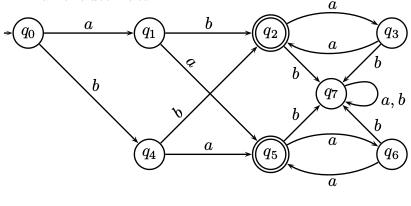
\includegraphics[width=0.8\textwidth]{afd_47_enunciado.png}
	\caption{Autómata del enunciado}
\end{figure}

Podemos ver claramente que $q_1 \equiv q_4$, $q_2 \equiv q_5$ y $q_3 \equiv q_6$. Este es el autómata minimizado:

\begin{figure}[H]
	\centering
	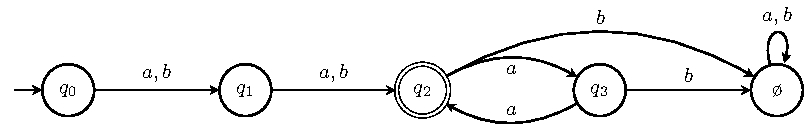
\includegraphics[width=0.8\textwidth]{afd_47.pdf}
	\caption{Autómata minimizado}
\end{figure}

\end{document}